\documentclass[1p]{elsarticle_modified}
%\bibliographystyle{elsarticle-num}

%\usepackage[colorlinks]{hyperref}
%\usepackage{abbrmath_seonhwa} %\Abb, \Ascr, \Acal ,\Abf, \Afrak
\usepackage{amsfonts}
\usepackage{amssymb}
\usepackage{amsmath}
\usepackage{amsthm}
\usepackage{scalefnt}
\usepackage{amsbsy}
\usepackage{kotex}
\usepackage{caption}
\usepackage{subfig}
\usepackage{color}
\usepackage{graphicx}
\usepackage{xcolor} %% white, black, red, green, blue, cyan, magenta, yellow
\usepackage{float}
\usepackage{setspace}
\usepackage{hyperref}

\usepackage{tikz}
\usetikzlibrary{arrows}

\usepackage{multirow}
\usepackage{array} % fixed length table
\usepackage{hhline}

%%%%%%%%%%%%%%%%%%%%%
\makeatletter
\renewcommand*\env@matrix[1][\arraystretch]{%
	\edef\arraystretch{#1}%
	\hskip -\arraycolsep
	\let\@ifnextchar\new@ifnextchar
	\array{*\c@MaxMatrixCols c}}
\makeatother %https://tex.stackexchange.com/questions/14071/how-can-i-increase-the-line-spacing-in-a-matrix
%%%%%%%%%%%%%%%

\usepackage[normalem]{ulem}

\newcommand{\msout}[1]{\ifmmode\text{\sout{\ensuremath{#1}}}\else\sout{#1}\fi}
%SOURCE: \msout is \stkout macro in https://tex.stackexchange.com/questions/20609/strikeout-in-math-mode

\newcommand{\cancel}[1]{
	\ifmmode
	{\color{red}\msout{#1}}
	\else
	{\color{red}\sout{#1}}
	\fi
}

\newcommand{\add}[1]{
	{\color{blue}\uwave{#1}}
}

\newcommand{\replace}[2]{
	\ifmmode
	{\color{red}\msout{#1}}{\color{blue}\uwave{#2}}
	\else
	{\color{red}\sout{#1}}{\color{blue}\uwave{#2}}
	\fi
}

\newcommand{\Sol}{\mathcal{S}} %segment
\newcommand{\D}{D} %diagram
\newcommand{\A}{\mathcal{A}} %arc


%%%%%%%%%%%%%%%%%%%%%%%%%%%%%5 test

\def\sl{\operatorname{\textup{SL}}(2,\Cbb)}
\def\psl{\operatorname{\textup{PSL}}(2,\Cbb)}
\def\quan{\mkern 1mu \triangleright \mkern 1mu}

\theoremstyle{definition}
\newtheorem{thm}{Theorem}[section]
\newtheorem{prop}[thm]{Proposition}
\newtheorem{lem}[thm]{Lemma}
\newtheorem{ques}[thm]{Question}
\newtheorem{cor}[thm]{Corollary}
\newtheorem{defn}[thm]{Definition}
\newtheorem{exam}[thm]{Example}
\newtheorem{rmk}[thm]{Remark}
\newtheorem{alg}[thm]{Algorithm}

\newcommand{\I}{\sqrt{-1}}
\begin{document}

%\begin{frontmatter}
%
%\title{Boundary parabolic representations of knots up to 8 crossings}
%
%%% Group authors per affiliation:
%\author{Yunhi Cho} 
%\address{Department of Mathematics, University of Seoul, Seoul, Korea}
%\ead{yhcho@uos.ac.kr}
%
%
%\author{Seonhwa Kim} %\fnref{s_kim}}
%\address{Center for Geometry and Physics, Institute for Basic Science, Pohang, 37673, Korea}
%\ead{ryeona17@ibs.re.kr}
%
%\author{Hyuk Kim}
%\address{Department of Mathematical Sciences, Seoul National University, Seoul 08826, Korea}
%\ead{hyukkim@snu.ac.kr}
%
%\author{Seokbeom Yoon}
%\address{Department of Mathematical Sciences, Seoul National University, Seoul, 08826,  Korea}
%\ead{sbyoon15@snu.ac.kr}
%
%\begin{abstract}
%We find all boundary parabolic representation of knots up to 8 crossings.
%
%\end{abstract}
%\begin{keyword}
%    \MSC[2010] 57M25 
%\end{keyword}
%
%\end{frontmatter}

%\linenumbers
%\tableofcontents
%
\newcommand\colored[1]{\textcolor{white}{\rule[-0.35ex]{0.8em}{1.4ex}}\kern-0.8em\color{red} #1}%
%\newcommand\colored[1]{\textcolor{white}{ #1}\kern-2.17ex	\textcolor{white}{ #1}\kern-1.81ex	\textcolor{white}{ #1}\kern-2.15ex\color{red}#1	}

{\Large $\underline{12a_{0068}~(K12a_{0068})}$}

\setlength{\tabcolsep}{10pt}
\renewcommand{\arraystretch}{1.6}
\vspace{1cm}\begin{tabular}{m{100pt}>{\centering\arraybackslash}m{274pt}}
\multirow{5}{120pt}{
	\centering
	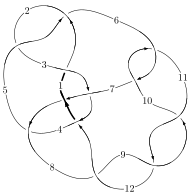
\includegraphics[width=112pt]{../../../GIT/diagram.site/Diagrams/png/869_12a_0068.png}\\
\ \ \ A knot diagram\footnotemark}&
\allowdisplaybreaks
\textbf{Linearized knot diagam} \\
\cline{2-2}
 &
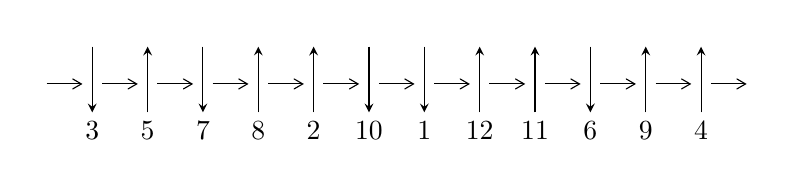
\begin{tikzpicture}[x=20pt, y=17pt]
	% nodes
	\node (C0) at (0, 0) {};
	\node (C1) at (1, 0) {};
	\node (C1U) at (1, +1) {};
	\node (C1D) at (1, -1) {3};

	\node (C2) at (2, 0) {};
	\node (C2U) at (2, +1) {};
	\node (C2D) at (2, -1) {5};

	\node (C3) at (3, 0) {};
	\node (C3U) at (3, +1) {};
	\node (C3D) at (3, -1) {7};

	\node (C4) at (4, 0) {};
	\node (C4U) at (4, +1) {};
	\node (C4D) at (4, -1) {8};

	\node (C5) at (5, 0) {};
	\node (C5U) at (5, +1) {};
	\node (C5D) at (5, -1) {2};

	\node (C6) at (6, 0) {};
	\node (C6U) at (6, +1) {};
	\node (C6D) at (6, -1) {10};

	\node (C7) at (7, 0) {};
	\node (C7U) at (7, +1) {};
	\node (C7D) at (7, -1) {1};

	\node (C8) at (8, 0) {};
	\node (C8U) at (8, +1) {};
	\node (C8D) at (8, -1) {12};

	\node (C9) at (9, 0) {};
	\node (C9U) at (9, +1) {};
	\node (C9D) at (9, -1) {11};

	\node (C10) at (10, 0) {};
	\node (C10U) at (10, +1) {};
	\node (C10D) at (10, -1) {6};

	\node (C11) at (11, 0) {};
	\node (C11U) at (11, +1) {};
	\node (C11D) at (11, -1) {9};

	\node (C12) at (12, 0) {};
	\node (C12U) at (12, +1) {};
	\node (C12D) at (12, -1) {4};
	\node (C13) at (13, 0) {};

	% arrows
	\draw[->,>={angle 60}]
	(C0) edge (C1) (C1) edge (C2) (C2) edge (C3) (C3) edge (C4) (C4) edge (C5) (C5) edge (C6) (C6) edge (C7) (C7) edge (C8) (C8) edge (C9) (C9) edge (C10) (C10) edge (C11) (C11) edge (C12) (C12) edge (C13) ;	\draw[->,>=stealth]
	(C1U) edge (C1D) (C2D) edge (C2U) (C3U) edge (C3D) (C4D) edge (C4U) (C5D) edge (C5U) (C6U) edge (C6D) (C7U) edge (C7D) (C8D) edge (C8U) (C9D) edge (C9U) (C10U) edge (C10D) (C11D) edge (C11U) (C12D) edge (C12U) ;
	\end{tikzpicture} \\
\hhline{~~} \\& 
\textbf{Solving Sequence} \\ \cline{2-2} 
 &
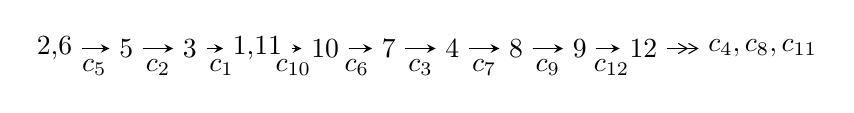
\begin{tikzpicture}[x=23pt, y=7pt]
	% node
	\node (A0) at (-1/8, 0) {2,6};
	\node (A1) at (1, 0) {5};
	\node (A2) at (2, 0) {3};
	\node (A3) at (49/16, 0) {1,11};
	\node (A4) at (33/8, 0) {10};
	\node (A5) at (41/8, 0) {7};
	\node (A6) at (49/8, 0) {4};
	\node (A7) at (57/8, 0) {8};
	\node (A8) at (65/8, 0) {9};
	\node (A9) at (73/8, 0) {12};
	\node (C1) at (1/2, -1) {$c_{5}$};
	\node (C2) at (3/2, -1) {$c_{2}$};
	\node (C3) at (5/2, -1) {$c_{1}$};
	\node (C4) at (29/8, -1) {$c_{10}$};
	\node (C5) at (37/8, -1) {$c_{6}$};
	\node (C6) at (45/8, -1) {$c_{3}$};
	\node (C7) at (53/8, -1) {$c_{7}$};
	\node (C8) at (61/8, -1) {$c_{9}$};
	\node (C9) at (69/8, -1) {$c_{12}$};
	\node (A10) at (11, 0) {$c_{4},c_{8},c_{11}$};

	% edge
	\draw[->,>=stealth]	
	(A0) edge (A1) (A1) edge (A2) (A2) edge (A3) (A3) edge (A4) (A4) edge (A5) (A5) edge (A6) (A6) edge (A7) (A7) edge (A8) (A8) edge (A9) ;
	\draw[->>,>={angle 60}]	
	(A9) edge (A10);
\end{tikzpicture} \\ 

\end{tabular} \\

\footnotetext{
The image of knot diagram is generated by the software ``\textbf{Draw programme}" developed by Andrew Bartholomew(\url{http://www.layer8.co.uk/maths/draw/index.htm\#Running-draw}), where we modified some parts for our purpose(\url{https://github.com/CATsTAILs/LinksPainter}).
}\phantom \\ \newline 
\centering \textbf{Ideals for irreducible components\footnotemark of $X_{\text{par}}$} 
 
\begin{align*}
I^u_{1}&=\langle 
1.25458\times10^{127} u^{95}+1.26518\times10^{128} u^{94}+\cdots+9.52869\times10^{127} b+1.50191\times10^{127},\\
\phantom{I^u_{1}}&\phantom{= \langle  }-9.57034\times10^{127} u^{95}-2.86258\times10^{128} u^{94}+\cdots+9.52869\times10^{127} a-2.12222\times10^{128},\\
\phantom{I^u_{1}}&\phantom{= \langle  }u^{96}+3 u^{95}+\cdots+12 u+1\rangle \\
I^u_{2}&=\langle 
b+u-1,\;a+u+2,\;u^2- u+1\rangle \\
I^u_{3}&=\langle 
b- u,\;a+1,\;u^2- u+1\rangle \\
\\
\end{align*}
\raggedright * 3 irreducible components of $\dim_{\mathbb{C}}=0$, with total 100 representations.\\
\footnotetext{All coefficients of polynomials are rational numbers. But the coefficients are sometimes approximated in decimal forms when there is not enough margin.}
\newpage
\renewcommand{\arraystretch}{1}
\centering \section*{I. $I^u_{1}= \langle 1.25\times10^{127} u^{95}+1.27\times10^{128} u^{94}+\cdots+9.53\times10^{127} b+1.50\times10^{127},\;-9.57\times10^{127} u^{95}-2.86\times10^{128} u^{94}+\cdots+9.53\times10^{127} a-2.12\times10^{128},\;u^{96}+3 u^{95}+\cdots+12 u+1 \rangle$}
\flushleft \textbf{(i) Arc colorings}\\
\begin{tabular}{m{7pt} m{180pt} m{7pt} m{180pt} }
\flushright $a_{2}=$&$\begin{pmatrix}0\\u\end{pmatrix}$ \\
\flushright $a_{6}=$&$\begin{pmatrix}1\\0\end{pmatrix}$ \\
\flushright $a_{5}=$&$\begin{pmatrix}1\\u^2\end{pmatrix}$ \\
\flushright $a_{3}=$&$\begin{pmatrix}u\\u^3+u\end{pmatrix}$ \\
\flushright $a_{1}=$&$\begin{pmatrix}u^3\\u^5+u^3+u\end{pmatrix}$ \\
\flushright $a_{11}=$&$\begin{pmatrix}1.00437 u^{95}+3.00416 u^{94}+\cdots+57.6273 u+2.22719\\-0.131664 u^{95}-1.32776 u^{94}+\cdots+1.94631 u-0.157620\end{pmatrix}$ \\
\flushright $a_{10}=$&$\begin{pmatrix}0.872707 u^{95}+1.67640 u^{94}+\cdots+59.5736 u+2.06957\\-0.131664 u^{95}-1.32776 u^{94}+\cdots+1.94631 u-0.157620\end{pmatrix}$ \\
\flushright $a_{7}=$&$\begin{pmatrix}1.95072 u^{95}+4.88246 u^{94}+\cdots-40.0809 u-3.74504\\0.869545 u^{95}+3.48417 u^{94}+\cdots+12.2237 u+0.518555\end{pmatrix}$ \\
\flushright $a_{4}=$&$\begin{pmatrix}0.309695 u^{95}+1.02345 u^{94}+\cdots+66.7347 u+5.22501\\0.403210 u^{95}+1.10905 u^{94}+\cdots+7.08302 u+0.778016\end{pmatrix}$ \\
\flushright $a_{8}=$&$\begin{pmatrix}0.687164 u^{95}-1.47942 u^{94}+\cdots-74.5773 u-6.69637\\2.39982 u^{95}+8.28580 u^{94}+\cdots+30.7068 u+2.07039\end{pmatrix}$ \\
\flushright $a_{9}=$&$\begin{pmatrix}-0.720528 u^{95}-2.13313 u^{94}+\cdots+43.6793 u+3.49267\\0.168650 u^{95}-0.178593 u^{94}+\cdots+0.999858 u+0.256902\end{pmatrix}$ \\
\flushright $a_{12}=$&$\begin{pmatrix}-0.248630 u^{95}-1.76800 u^{94}+\cdots-10.1284 u-1.85496\\0.900641 u^{95}+2.78697 u^{94}+\cdots+16.1924 u+1.08286\end{pmatrix}$\\&\end{tabular}
\flushleft \textbf{(ii) Obstruction class $= -1$}\\~\\
\flushleft \textbf{(iii) Cusp Shapes $= -4.65162 u^{95}-10.5791 u^{94}+\cdots-96.8246 u-7.50867$}\\~\\
\newpage\renewcommand{\arraystretch}{1}
\flushleft \textbf{(iv) u-Polynomials at the component}\newline \\
\begin{tabular}{m{50pt}|m{274pt}}
Crossings & \hspace{64pt}u-Polynomials at each crossing \\
\hline $$\begin{aligned}c_{1}\end{aligned}$$&$\begin{aligned}
&u^{96}+43 u^{95}+\cdots+80 u+1
\end{aligned}$\\
\hline $$\begin{aligned}c_{2},c_{5}\end{aligned}$$&$\begin{aligned}
&u^{96}+3 u^{95}+\cdots+12 u+1
\end{aligned}$\\
\hline $$\begin{aligned}c_{3}\end{aligned}$$&$\begin{aligned}
&u^{96}+42 u^{94}+\cdots+1035 u+643
\end{aligned}$\\
\hline $$\begin{aligned}c_{4}\end{aligned}$$&$\begin{aligned}
&u^{96}-2 u^{95}+\cdots+13621 u+1921
\end{aligned}$\\
\hline $$\begin{aligned}c_{6},c_{10}\end{aligned}$$&$\begin{aligned}
&u^{96}+3 u^{95}+\cdots-2 u+1
\end{aligned}$\\
\hline $$\begin{aligned}c_{7}\end{aligned}$$&$\begin{aligned}
&u^{96}-7 u^{95}+\cdots+4 u^2+1
\end{aligned}$\\
\hline $$\begin{aligned}c_{8},c_{9},c_{11}\end{aligned}$$&$\begin{aligned}
&u^{96}-23 u^{95}+\cdots-8 u+1
\end{aligned}$\\
\hline $$\begin{aligned}c_{12}\end{aligned}$$&$\begin{aligned}
&u^{96}+9 u^{95}+\cdots-16 u+16
\end{aligned}$\\
\hline
\end{tabular}\\~\\
\newpage\renewcommand{\arraystretch}{1}
\flushleft \textbf{(v) Riley Polynomials at the component}\newline \\
\begin{tabular}{m{50pt}|m{274pt}}
Crossings & \hspace{64pt}Riley Polynomials at each crossing \\
\hline $$\begin{aligned}c_{1}\end{aligned}$$&$\begin{aligned}
&y^{96}+23 y^{95}+\cdots-1248 y+1
\end{aligned}$\\
\hline $$\begin{aligned}c_{2},c_{5}\end{aligned}$$&$\begin{aligned}
&y^{96}+43 y^{95}+\cdots+80 y+1
\end{aligned}$\\
\hline $$\begin{aligned}c_{3}\end{aligned}$$&$\begin{aligned}
&y^{96}+84 y^{95}+\cdots-13909363 y+413449
\end{aligned}$\\
\hline $$\begin{aligned}c_{4}\end{aligned}$$&$\begin{aligned}
&y^{96}+116 y^{95}+\cdots+95698917 y+3690241
\end{aligned}$\\
\hline $$\begin{aligned}c_{6},c_{10}\end{aligned}$$&$\begin{aligned}
&y^{96}+23 y^{95}+\cdots+8 y+1
\end{aligned}$\\
\hline $$\begin{aligned}c_{7}\end{aligned}$$&$\begin{aligned}
&y^{96}+11 y^{95}+\cdots+8 y+1
\end{aligned}$\\
\hline $$\begin{aligned}c_{8},c_{9},c_{11}\end{aligned}$$&$\begin{aligned}
&y^{96}+103 y^{95}+\cdots-48 y+1
\end{aligned}$\\
\hline $$\begin{aligned}c_{12}\end{aligned}$$&$\begin{aligned}
&y^{96}+25 y^{95}+\cdots+2944 y+256
\end{aligned}$\\
\hline
\end{tabular}\\~\\
\newpage\flushleft \textbf{(vi) Complex Volumes and Cusp Shapes}
$$\begin{array}{c|c|c}  
\text{Solutions to }I^u_{1}& \I (\text{vol} + \sqrt{-1}CS) & \text{Cusp shape}\\
 \hline 
\begin{aligned}
u &= -0.944130 + 0.380710 I \\
a &= \phantom{-}0.747578 + 0.125727 I \\
b &= -0.899713 - 0.842502 I\end{aligned}
 & -6.40890 + 5.50823 I & \phantom{-0.000000 } 0 \\ \hline\begin{aligned}
u &= -0.944130 - 0.380710 I \\
a &= \phantom{-}0.747578 - 0.125727 I \\
b &= -0.899713 + 0.842502 I\end{aligned}
 & -6.40890 - 5.50823 I & \phantom{-0.000000 } 0 \\ \hline\begin{aligned}
u &= \phantom{-}0.443410 + 0.868939 I \\
a &= \phantom{-}1.09874 + 3.16937 I \\
b &= -0.391123 - 0.642425 I\end{aligned}
 & -0.163424 + 0.651132 I & \phantom{-0.000000 } 0 \\ \hline\begin{aligned}
u &= \phantom{-}0.443410 - 0.868939 I \\
a &= \phantom{-}1.09874 - 3.16937 I \\
b &= -0.391123 + 0.642425 I\end{aligned}
 & -0.163424 - 0.651132 I & \phantom{-0.000000 } 0 \\ \hline\begin{aligned}
u &= -0.857554 + 0.459267 I \\
a &= -0.544829 - 1.001310 I \\
b &= \phantom{-}0.425826 - 0.982792 I\end{aligned}
 & \phantom{-}2.25759 + 7.89368 I & \phantom{-0.000000 } 0 \\ \hline\begin{aligned}
u &= -0.857554 - 0.459267 I \\
a &= -0.544829 + 1.001310 I \\
b &= \phantom{-}0.425826 + 0.982792 I\end{aligned}
 & \phantom{-}2.25759 - 7.89368 I & \phantom{-0.000000 } 0 \\ \hline\begin{aligned}
u &= \phantom{-}1.027200 + 0.030408 I \\
a &= \phantom{-}1.251760 + 0.113225 I \\
b &= -0.821562 - 0.901812 I\end{aligned}
 & -2.85315 - 3.06998 I & \phantom{-0.000000 } 0 \\ \hline\begin{aligned}
u &= \phantom{-}1.027200 - 0.030408 I \\
a &= \phantom{-}1.251760 - 0.113225 I \\
b &= -0.821562 + 0.901812 I\end{aligned}
 & -2.85315 + 3.06998 I & \phantom{-0.000000 } 0 \\ \hline\begin{aligned}
u &= \phantom{-}0.511371 + 0.891488 I \\
a &= \phantom{-}4.81043 + 2.73170 I \\
b &= -0.366736 + 0.764497 I\end{aligned}
 & \phantom{-}0.22700 + 3.68030 I & \phantom{-0.000000 } 0 \\ \hline\begin{aligned}
u &= \phantom{-}0.511371 - 0.891488 I \\
a &= \phantom{-}4.81043 - 2.73170 I \\
b &= -0.366736 - 0.764497 I\end{aligned}
 & \phantom{-}0.22700 - 3.68030 I & \phantom{-0.000000 } 0\\
 \hline 
 \end{array}$$\newpage$$\begin{array}{c|c|c}  
\text{Solutions to }I^u_{1}& \I (\text{vol} + \sqrt{-1}CS) & \text{Cusp shape}\\
 \hline 
\begin{aligned}
u &= -0.954773 + 0.399875 I \\
a &= \phantom{-}1.114810 + 0.371359 I \\
b &= -0.838711 + 0.981826 I\end{aligned}
 & -5.96628 + 11.93610 I & \phantom{-0.000000 } 0 \\ \hline\begin{aligned}
u &= -0.954773 - 0.399875 I \\
a &= \phantom{-}1.114810 - 0.371359 I \\
b &= -0.838711 - 0.981826 I\end{aligned}
 & -5.96628 - 11.93610 I & \phantom{-0.000000 } 0 \\ \hline\begin{aligned}
u &= \phantom{-}0.495783 + 0.817895 I \\
a &= \phantom{-}0.47218 - 3.80289 I \\
b &= -0.304347 - 0.764185 I\end{aligned}
 & \phantom{-}0.474880 + 0.427443 I & \phantom{-0.000000 } 0 \\ \hline\begin{aligned}
u &= \phantom{-}0.495783 - 0.817895 I \\
a &= \phantom{-}0.47218 + 3.80289 I \\
b &= -0.304347 + 0.764185 I\end{aligned}
 & \phantom{-}0.474880 - 0.427443 I & \phantom{-0.000000 } 0 \\ \hline\begin{aligned}
u &= \phantom{-}0.442328 + 0.966095 I \\
a &= -0.188046 - 0.726355 I \\
b &= -0.206747 + 0.360314 I\end{aligned}
 & -0.42331 + 2.75224 I & \phantom{-0.000000 } 0 \\ \hline\begin{aligned}
u &= \phantom{-}0.442328 - 0.966095 I \\
a &= -0.188046 + 0.726355 I \\
b &= -0.206747 - 0.360314 I\end{aligned}
 & -0.42331 - 2.75224 I & \phantom{-0.000000 } 0 \\ \hline\begin{aligned}
u &= -0.435286 + 0.975110 I \\
a &= \phantom{-}1.84603 - 0.96584 I \\
b &= -0.378271 - 1.055990 I\end{aligned}
 & -0.93138 - 4.78594 I & \phantom{-0.000000 } 0 \\ \hline\begin{aligned}
u &= -0.435286 - 0.975110 I \\
a &= \phantom{-}1.84603 + 0.96584 I \\
b &= -0.378271 + 1.055990 I\end{aligned}
 & -0.93138 + 4.78594 I & \phantom{-0.000000 } 0 \\ \hline\begin{aligned}
u &= -0.335424 + 1.022430 I \\
a &= \phantom{-}0.633874 - 0.863645 I \\
b &= -0.714957 + 0.191046 I\end{aligned}
 & -3.72797 - 0.83654 I & \phantom{-0.000000 } 0 \\ \hline\begin{aligned}
u &= -0.335424 - 1.022430 I \\
a &= \phantom{-}0.633874 + 0.863645 I \\
b &= -0.714957 - 0.191046 I\end{aligned}
 & -3.72797 + 0.83654 I & \phantom{-0.000000 } 0\\
 \hline 
 \end{array}$$\newpage$$\begin{array}{c|c|c}  
\text{Solutions to }I^u_{1}& \I (\text{vol} + \sqrt{-1}CS) & \text{Cusp shape}\\
 \hline 
\begin{aligned}
u &= \phantom{-}0.885662 + 0.616135 I \\
a &= -0.792115 - 1.026420 I \\
b &= \phantom{-}0.302376 - 0.842845 I\end{aligned}
 & \phantom{-}2.96137 + 3.75608 I & \phantom{-0.000000 } 0 \\ \hline\begin{aligned}
u &= \phantom{-}0.885662 - 0.616135 I \\
a &= -0.792115 + 1.026420 I \\
b &= \phantom{-}0.302376 + 0.842845 I\end{aligned}
 & \phantom{-}2.96137 - 3.75608 I & \phantom{-0.000000 } 0 \\ \hline\begin{aligned}
u &= \phantom{-}0.481557 + 0.972545 I \\
a &= -0.28450 - 3.24363 I \\
b &= \phantom{-}0.858693 + 0.897946 I\end{aligned}
 & -7.09470 - 0.51155 I & \phantom{-0.000000 } 0 \\ \hline\begin{aligned}
u &= \phantom{-}0.481557 - 0.972545 I \\
a &= -0.28450 + 3.24363 I \\
b &= \phantom{-}0.858693 - 0.897946 I\end{aligned}
 & -7.09470 + 0.51155 I & \phantom{-0.000000 } 0 \\ \hline\begin{aligned}
u &= \phantom{-}0.848669 + 0.330833 I \\
a &= -0.869068 + 0.875953 I \\
b &= \phantom{-}0.249847 + 0.830961 I\end{aligned}
 & \phantom{-}3.22915 - 0.49581 I & \phantom{-0.000000 } 0 \\ \hline\begin{aligned}
u &= \phantom{-}0.848669 - 0.330833 I \\
a &= -0.869068 - 0.875953 I \\
b &= \phantom{-}0.249847 - 0.830961 I\end{aligned}
 & \phantom{-}3.22915 + 0.49581 I & \phantom{-0.000000 } 0 \\ \hline\begin{aligned}
u &= \phantom{-}0.496910 + 0.969309 I \\
a &= -4.30112 - 0.91811 I \\
b &= \phantom{-}0.847726 - 0.924734 I\end{aligned}
 & -7.00971 + 5.82431 I & \phantom{-0.000000 } 0 \\ \hline\begin{aligned}
u &= \phantom{-}0.496910 - 0.969309 I \\
a &= -4.30112 + 0.91811 I \\
b &= \phantom{-}0.847726 + 0.924734 I\end{aligned}
 & -7.00971 - 5.82431 I & \phantom{-0.000000 } 0 \\ \hline\begin{aligned}
u &= -0.307628 + 1.048570 I \\
a &= -1.38854 + 1.25263 I \\
b &= \phantom{-}0.882149 - 0.968150 I\end{aligned}
 & -10.51930 + 2.73208 I & \phantom{-0.000000 } 0 \\ \hline\begin{aligned}
u &= -0.307628 - 1.048570 I \\
a &= -1.38854 - 1.25263 I \\
b &= \phantom{-}0.882149 + 0.968150 I\end{aligned}
 & -10.51930 - 2.73208 I & \phantom{-0.000000 } 0\\
 \hline 
 \end{array}$$\newpage$$\begin{array}{c|c|c}  
\text{Solutions to }I^u_{1}& \I (\text{vol} + \sqrt{-1}CS) & \text{Cusp shape}\\
 \hline 
\begin{aligned}
u &= -0.501616 + 0.982193 I \\
a &= \phantom{-}0.352505 - 0.078570 I \\
b &= -0.538847 + 1.044320 I\end{aligned}
 & -0.517012 - 0.811673 I & \phantom{-0.000000 } 0 \\ \hline\begin{aligned}
u &= -0.501616 - 0.982193 I \\
a &= \phantom{-}0.352505 + 0.078570 I \\
b &= -0.538847 - 1.044320 I\end{aligned}
 & -0.517012 + 0.811673 I & \phantom{-0.000000 } 0 \\ \hline\begin{aligned}
u &= -0.716350 + 0.537726 I \\
a &= -0.74398 + 1.45731 I \\
b &= \phantom{-}0.067086 + 0.995847 I\end{aligned}
 & \phantom{-}4.33816 + 2.12439 I & \phantom{-0.000000 } 0 \\ \hline\begin{aligned}
u &= -0.716350 - 0.537726 I \\
a &= -0.74398 - 1.45731 I \\
b &= \phantom{-}0.067086 - 0.995847 I\end{aligned}
 & \phantom{-}4.33816 - 2.12439 I & \phantom{-0.000000 } 0 \\ \hline\begin{aligned}
u &= -0.336126 + 1.063530 I \\
a &= -2.21471 - 0.40695 I \\
b &= \phantom{-}0.921333 + 0.890200 I\end{aligned}
 & -10.77110 - 3.90533 I & \phantom{-0.000000 } 0 \\ \hline\begin{aligned}
u &= -0.336126 - 1.063530 I \\
a &= -2.21471 + 0.40695 I \\
b &= \phantom{-}0.921333 - 0.890200 I\end{aligned}
 & -10.77110 + 3.90533 I & \phantom{-0.000000 } 0 \\ \hline\begin{aligned}
u &= -0.786461 + 0.400210 I \\
a &= -0.453433 + 0.190964 I \\
b &= \phantom{-}0.683514 + 0.292441 I\end{aligned}
 & \phantom{-}0.06293 + 3.86040 I & \phantom{-0.000000 } 0 \\ \hline\begin{aligned}
u &= -0.786461 - 0.400210 I \\
a &= -0.453433 - 0.190964 I \\
b &= \phantom{-}0.683514 - 0.292441 I\end{aligned}
 & \phantom{-}0.06293 - 3.86040 I & \phantom{-0.000000 } 0 \\ \hline\begin{aligned}
u &= -0.248408 + 0.815682 I \\
a &= -0.620667 + 0.770716 I \\
b &= -0.215599 + 0.978033 I\end{aligned}
 & \phantom{-}0.03402 + 1.62772 I & \phantom{-0.000000 } 0. - 5.83773 I \\ \hline\begin{aligned}
u &= -0.248408 - 0.815682 I \\
a &= -0.620667 - 0.770716 I \\
b &= -0.215599 - 0.978033 I\end{aligned}
 & \phantom{-}0.03402 - 1.62772 I & \phantom{-0.000000 -}0. + 5.83773 I\\
 \hline 
 \end{array}$$\newpage$$\begin{array}{c|c|c}  
\text{Solutions to }I^u_{1}& \I (\text{vol} + \sqrt{-1}CS) & \text{Cusp shape}\\
 \hline 
\begin{aligned}
u &= -0.131774 + 1.152770 I \\
a &= -1.45241 - 0.17244 I \\
b &= \phantom{-}0.652615 + 0.482184 I\end{aligned}
 & -5.04933 + 1.45448 I & \phantom{-0.000000 } 0 \\ \hline\begin{aligned}
u &= -0.131774 - 1.152770 I \\
a &= -1.45241 + 0.17244 I \\
b &= \phantom{-}0.652615 - 0.482184 I\end{aligned}
 & -5.04933 - 1.45448 I & \phantom{-0.000000 } 0 \\ \hline\begin{aligned}
u &= \phantom{-}0.618669 + 0.564064 I \\
a &= -0.731160 + 0.168587 I \\
b &= \phantom{-}0.337857 + 0.044079 I\end{aligned}
 & \phantom{-}1.11274 + 1.43343 I & \phantom{-0.000000 } 0 \\ \hline\begin{aligned}
u &= \phantom{-}0.618669 - 0.564064 I \\
a &= -0.731160 - 0.168587 I \\
b &= \phantom{-}0.337857 - 0.044079 I\end{aligned}
 & \phantom{-}1.11274 - 1.43343 I & \phantom{-0.000000 } 0 \\ \hline\begin{aligned}
u &= -0.486797 + 0.675531 I \\
a &= \phantom{-}2.08735 - 1.12575 I \\
b &= -0.605434 - 0.973948 I\end{aligned}
 & \phantom{-}0.48275 - 3.26120 I & \phantom{-0.000000 } 0 \\ \hline\begin{aligned}
u &= -0.486797 - 0.675531 I \\
a &= \phantom{-}2.08735 + 1.12575 I \\
b &= -0.605434 + 0.973948 I\end{aligned}
 & \phantom{-}0.48275 + 3.26120 I & \phantom{-0.000000 } 0 \\ \hline\begin{aligned}
u &= -0.515401 + 1.049240 I \\
a &= \phantom{-}1.234010 - 0.202961 I \\
b &= -0.795511 - 0.414270 I\end{aligned}
 & -2.53671 - 5.70933 I & \phantom{-0.000000 } 0 \\ \hline\begin{aligned}
u &= -0.515401 - 1.049240 I \\
a &= \phantom{-}1.234010 + 0.202961 I \\
b &= -0.795511 + 0.414270 I\end{aligned}
 & -2.53671 + 5.70933 I & \phantom{-0.000000 } 0 \\ \hline\begin{aligned}
u &= \phantom{-}0.494599 + 0.643086 I \\
a &= -1.04179 + 1.56013 I \\
b &= \phantom{-}0.833613 + 0.904001 I\end{aligned}
 & -6.02813 - 1.72993 I & -7.66096 + 0. I\phantom{ +0.000000I} \\ \hline\begin{aligned}
u &= \phantom{-}0.494599 - 0.643086 I \\
a &= -1.04179 - 1.56013 I \\
b &= \phantom{-}0.833613 - 0.904001 I\end{aligned}
 & -6.02813 + 1.72993 I & -7.66096 + 0. I\phantom{ +0.000000I}\\
 \hline 
 \end{array}$$\newpage$$\begin{array}{c|c|c}  
\text{Solutions to }I^u_{1}& \I (\text{vol} + \sqrt{-1}CS) & \text{Cusp shape}\\
 \hline 
\begin{aligned}
u &= -0.520441 + 1.079590 I \\
a &= -2.50628 + 0.70243 I \\
b &= \phantom{-}0.833253 + 1.003160 I\end{aligned}
 & -9.09740 - 9.67597 I & \phantom{-0.000000 } 0 \\ \hline\begin{aligned}
u &= -0.520441 - 1.079590 I \\
a &= -2.50628 - 0.70243 I \\
b &= \phantom{-}0.833253 - 1.003160 I\end{aligned}
 & -9.09740 + 9.67597 I & \phantom{-0.000000 } 0 \\ \hline\begin{aligned}
u &= -0.497538 + 1.092080 I \\
a &= -0.40904 + 1.48452 I \\
b &= \phantom{-}0.914869 - 0.818882 I\end{aligned}
 & -9.68241 - 3.22210 I & \phantom{-0.000000 } 0 \\ \hline\begin{aligned}
u &= -0.497538 - 1.092080 I \\
a &= -0.40904 - 1.48452 I \\
b &= \phantom{-}0.914869 + 0.818882 I\end{aligned}
 & -9.68241 + 3.22210 I & \phantom{-0.000000 } 0 \\ \hline\begin{aligned}
u &= -0.603639 + 1.040350 I \\
a &= \phantom{-}0.712076 - 0.808224 I \\
b &= \phantom{-}0.024797 - 1.053490 I\end{aligned}
 & \phantom{-}2.83612 - 7.19113 I & \phantom{-0.000000 } 0 \\ \hline\begin{aligned}
u &= -0.603639 - 1.040350 I \\
a &= \phantom{-}0.712076 + 0.808224 I \\
b &= \phantom{-}0.024797 + 1.053490 I\end{aligned}
 & \phantom{-}2.83612 + 7.19113 I & \phantom{-0.000000 } 0 \\ \hline\begin{aligned}
u &= -0.008517 + 1.202810 I \\
a &= -1.171860 + 0.337612 I \\
b &= \phantom{-}0.495583 - 0.885320 I\end{aligned}
 & -3.75875 + 5.69385 I & \phantom{-0.000000 } 0 \\ \hline\begin{aligned}
u &= -0.008517 - 1.202810 I \\
a &= -1.171860 - 0.337612 I \\
b &= \phantom{-}0.495583 + 0.885320 I\end{aligned}
 & -3.75875 - 5.69385 I & \phantom{-0.000000 } 0 \\ \hline\begin{aligned}
u &= \phantom{-}0.521857 + 1.085650 I \\
a &= -0.694262 - 0.567269 I \\
b &= \phantom{-}0.362113 + 0.388664 I\end{aligned}
 & -0.46985 + 2.99535 I & \phantom{-0.000000 } 0 \\ \hline\begin{aligned}
u &= \phantom{-}0.521857 - 1.085650 I \\
a &= -0.694262 + 0.567269 I \\
b &= \phantom{-}0.362113 - 0.388664 I\end{aligned}
 & -0.46985 - 2.99535 I & \phantom{-0.000000 } 0\\
 \hline 
 \end{array}$$\newpage$$\begin{array}{c|c|c}  
\text{Solutions to }I^u_{1}& \I (\text{vol} + \sqrt{-1}CS) & \text{Cusp shape}\\
 \hline 
\begin{aligned}
u &= \phantom{-}0.724609 + 0.963903 I \\
a &= -0.147279 + 0.759365 I \\
b &= \phantom{-}0.177058 + 0.763394 I\end{aligned}
 & \phantom{-}1.92331 + 2.16760 I & \phantom{-0.000000 } 0 \\ \hline\begin{aligned}
u &= \phantom{-}0.724609 - 0.963903 I \\
a &= -0.147279 - 0.759365 I \\
b &= \phantom{-}0.177058 - 0.763394 I\end{aligned}
 & \phantom{-}1.92331 - 2.16760 I & \phantom{-0.000000 } 0 \\ \hline\begin{aligned}
u &= \phantom{-}0.466118 + 0.606924 I \\
a &= \phantom{-}0.376644 + 0.066273 I \\
b &= \phantom{-}0.831644 - 0.905874 I\end{aligned}
 & -6.02130 + 4.47862 I & -6.84478 - 6.25873 I \\ \hline\begin{aligned}
u &= \phantom{-}0.466118 - 0.606924 I \\
a &= \phantom{-}0.376644 - 0.066273 I \\
b &= \phantom{-}0.831644 + 0.905874 I\end{aligned}
 & -6.02130 - 4.47862 I & -6.84478 + 6.25873 I \\ \hline\begin{aligned}
u &= -0.600794 + 1.108700 I \\
a &= -0.615812 + 0.860511 I \\
b &= \phantom{-}0.763068 - 0.309131 I\end{aligned}
 & -2.02943 - 9.07322 I & \phantom{-0.000000 } 0 \\ \hline\begin{aligned}
u &= -0.600794 - 1.108700 I \\
a &= -0.615812 - 0.860511 I \\
b &= \phantom{-}0.763068 + 0.309131 I\end{aligned}
 & -2.02943 + 9.07322 I & \phantom{-0.000000 } 0 \\ \hline\begin{aligned}
u &= \phantom{-}0.981681 + 0.808812 I \\
a &= \phantom{-}1.44463 + 0.39076 I \\
b &= -0.824528 + 0.920065 I\end{aligned}
 & -3.67065 + 6.52415 I & \phantom{-0.000000 } 0 \\ \hline\begin{aligned}
u &= \phantom{-}0.981681 - 0.808812 I \\
a &= \phantom{-}1.44463 - 0.39076 I \\
b &= -0.824528 - 0.920065 I\end{aligned}
 & -3.67065 - 6.52415 I & \phantom{-0.000000 } 0 \\ \hline\begin{aligned}
u &= \phantom{-}0.962702 + 0.841959 I \\
a &= \phantom{-}0.705311 + 0.351305 I \\
b &= -0.834536 - 0.886420 I\end{aligned}
 & -3.77486 + 0.33567 I & \phantom{-0.000000 } 0 \\ \hline\begin{aligned}
u &= \phantom{-}0.962702 - 0.841959 I \\
a &= \phantom{-}0.705311 - 0.351305 I \\
b &= -0.834536 + 0.886420 I\end{aligned}
 & -3.77486 - 0.33567 I & \phantom{-0.000000 } 0\\
 \hline 
 \end{array}$$\newpage$$\begin{array}{c|c|c}  
\text{Solutions to }I^u_{1}& \I (\text{vol} + \sqrt{-1}CS) & \text{Cusp shape}\\
 \hline 
\begin{aligned}
u &= -0.642079 + 1.111450 I \\
a &= -1.86968 + 0.86375 I \\
b &= \phantom{-}0.452310 + 1.017020 I\end{aligned}
 & \phantom{-}0.28760 - 13.45100 I & \phantom{-0.000000 } 0 \\ \hline\begin{aligned}
u &= -0.642079 - 1.111450 I \\
a &= -1.86968 - 0.86375 I \\
b &= \phantom{-}0.452310 - 1.017020 I\end{aligned}
 & \phantom{-}0.28760 + 13.45100 I & \phantom{-0.000000 } 0 \\ \hline\begin{aligned}
u &= \phantom{-}0.653023 + 1.146890 I \\
a &= -1.71130 - 0.69568 I \\
b &= \phantom{-}0.377764 - 0.847444 I\end{aligned}
 & \phantom{-}0.84141 + 6.09074 I & \phantom{-0.000000 } 0 \\ \hline\begin{aligned}
u &= \phantom{-}0.653023 - 1.146890 I \\
a &= -1.71130 + 0.69568 I \\
b &= \phantom{-}0.377764 + 0.847444 I\end{aligned}
 & \phantom{-}0.84141 - 6.09074 I & \phantom{-0.000000 } 0 \\ \hline\begin{aligned}
u &= -0.602288 + 0.306455 I \\
a &= -0.500477 - 0.775423 I \\
b &= \phantom{-}0.829104 - 0.966580 I\end{aligned}
 & -6.94884 + 5.24603 I & -0.89797 - 3.65025 I \\ \hline\begin{aligned}
u &= -0.602288 - 0.306455 I \\
a &= -0.500477 + 0.775423 I \\
b &= \phantom{-}0.829104 + 0.966580 I\end{aligned}
 & -6.94884 - 5.24603 I & -0.89797 + 3.65025 I \\ \hline\begin{aligned}
u &= -0.643378 + 1.170880 I \\
a &= \phantom{-}0.49879 - 1.47590 I \\
b &= -0.917934 + 0.838845 I\end{aligned}
 & -8.8221 - 11.2866 I & \phantom{-0.000000 } 0 \\ \hline\begin{aligned}
u &= -0.643378 - 1.170880 I \\
a &= \phantom{-}0.49879 + 1.47590 I \\
b &= -0.917934 - 0.838845 I\end{aligned}
 & -8.8221 + 11.2866 I & \phantom{-0.000000 } 0 \\ \hline\begin{aligned}
u &= -0.654680 + 1.169780 I \\
a &= \phantom{-}2.50773 - 0.59269 I \\
b &= -0.845297 - 0.994247 I\end{aligned}
 & -8.3247 - 17.7909 I & \phantom{-0.000000 } 0 \\ \hline\begin{aligned}
u &= -0.654680 - 1.169780 I \\
a &= \phantom{-}2.50773 + 0.59269 I \\
b &= -0.845297 + 0.994247 I\end{aligned}
 & -8.3247 + 17.7909 I & \phantom{-0.000000 } 0\\
 \hline 
 \end{array}$$\newpage$$\begin{array}{c|c|c}  
\text{Solutions to }I^u_{1}& \I (\text{vol} + \sqrt{-1}CS) & \text{Cusp shape}\\
 \hline 
\begin{aligned}
u &= -0.106772 + 1.336530 I \\
a &= \phantom{-}1.94764 + 0.93501 I \\
b &= -0.895094 - 0.877393 I\end{aligned}
 & -12.53720 + 2.14016 I & \phantom{-0.000000 } 0 \\ \hline\begin{aligned}
u &= -0.106772 - 1.336530 I \\
a &= \phantom{-}1.94764 - 0.93501 I \\
b &= -0.895094 + 0.877393 I\end{aligned}
 & -12.53720 - 2.14016 I & \phantom{-0.000000 } 0 \\ \hline\begin{aligned}
u &= -0.608796 + 0.241383 I \\
a &= -0.260844 + 0.431600 I \\
b &= \phantom{-}0.878462 + 0.850220 I\end{aligned}
 & -7.31889 - 1.08877 I & -1.71710 + 1.55322 I \\ \hline\begin{aligned}
u &= -0.608796 - 0.241383 I \\
a &= -0.260844 - 0.431600 I \\
b &= \phantom{-}0.878462 - 0.850220 I\end{aligned}
 & -7.31889 + 1.08877 I & -1.71710 - 1.55322 I \\ \hline\begin{aligned}
u &= -0.085403 + 1.345550 I \\
a &= \phantom{-}1.94973 - 0.89454 I \\
b &= -0.857458 + 0.959884 I\end{aligned}
 & -12.2733 + 8.6180 I & \phantom{-0.000000 } 0 \\ \hline\begin{aligned}
u &= -0.085403 - 1.345550 I \\
a &= \phantom{-}1.94973 + 0.89454 I \\
b &= -0.857458 - 0.959884 I\end{aligned}
 & -12.2733 - 8.6180 I & \phantom{-0.000000 } 0 \\ \hline\begin{aligned}
u &= \phantom{-}0.590589 + 1.280660 I \\
a &= \phantom{-}1.03845 + 1.35814 I \\
b &= -0.859053 - 0.878861 I\end{aligned}
 & -6.71027 + 2.59153 I & \phantom{-0.000000 } 0 \\ \hline\begin{aligned}
u &= \phantom{-}0.590589 - 1.280660 I \\
a &= \phantom{-}1.03845 - 1.35814 I \\
b &= -0.859053 + 0.878861 I\end{aligned}
 & -6.71027 - 2.59153 I & \phantom{-0.000000 } 0 \\ \hline\begin{aligned}
u &= \phantom{-}0.61589 + 1.27907 I \\
a &= \phantom{-}2.40565 + 0.04727 I \\
b &= -0.837169 + 0.937778 I\end{aligned}
 & -6.52555 + 8.89397 I & \phantom{-0.000000 } 0 \\ \hline\begin{aligned}
u &= \phantom{-}0.61589 - 1.27907 I \\
a &= \phantom{-}2.40565 - 0.04727 I \\
b &= -0.837169 - 0.937778 I\end{aligned}
 & -6.52555 - 8.89397 I & \phantom{-0.000000 } 0\\
 \hline 
 \end{array}$$\newpage$$\begin{array}{c|c|c}  
\text{Solutions to }I^u_{1}& \I (\text{vol} + \sqrt{-1}CS) & \text{Cusp shape}\\
 \hline 
\begin{aligned}
u &= -0.397629 + 0.335038 I \\
a &= -0.446115 - 0.890174 I \\
b &= -0.617980 + 0.502353 I\end{aligned}
 & -0.69586 + 1.56046 I & -1.20236 - 4.38031 I \\ \hline\begin{aligned}
u &= -0.397629 - 0.335038 I \\
a &= -0.446115 + 0.890174 I \\
b &= -0.617980 - 0.502353 I\end{aligned}
 & -0.69586 - 1.56046 I & -1.20236 + 4.38031 I \\ \hline\begin{aligned}
u &= -0.190813 + 0.456129 I \\
a &= -0.26886 - 1.66079 I \\
b &= -0.597450 + 0.605363 I\end{aligned}
 & -0.67284 + 1.56655 I & -1.33932 - 5.04903 I \\ \hline\begin{aligned}
u &= -0.190813 - 0.456129 I \\
a &= -0.26886 + 1.66079 I \\
b &= -0.597450 - 0.605363 I\end{aligned}
 & -0.67284 - 1.56655 I & -1.33932 + 5.04903 I \\ \hline\begin{aligned}
u &= -0.042138 + 0.164105 I \\
a &= -3.50773 + 1.29660 I \\
b &= -0.338604 + 0.829605 I\end{aligned}
 & \phantom{-}0.35198 + 1.84473 I & \phantom{-}0.73666 - 4.91315 I \\ \hline\begin{aligned}
u &= -0.042138 - 0.164105 I \\
a &= -3.50773 - 1.29660 I \\
b &= -0.338604 - 0.829605 I\end{aligned}
 & \phantom{-}0.35198 - 1.84473 I & \phantom{-}0.73666 + 4.91315 I\\
 \hline 
 \end{array}$$\newpage\newpage\renewcommand{\arraystretch}{1}
\centering \section*{II. $I^u_{2}= \langle b+u-1,\;a+u+2,\;u^2- u+1 \rangle$}
\flushleft \textbf{(i) Arc colorings}\\
\begin{tabular}{m{7pt} m{180pt} m{7pt} m{180pt} }
\flushright $a_{2}=$&$\begin{pmatrix}0\\u\end{pmatrix}$ \\
\flushright $a_{6}=$&$\begin{pmatrix}1\\0\end{pmatrix}$ \\
\flushright $a_{5}=$&$\begin{pmatrix}1\\u-1\end{pmatrix}$ \\
\flushright $a_{3}=$&$\begin{pmatrix}u\\u-1\end{pmatrix}$ \\
\flushright $a_{1}=$&$\begin{pmatrix}-1\\0\end{pmatrix}$ \\
\flushright $a_{11}=$&$\begin{pmatrix}- u-2\\- u+1\end{pmatrix}$ \\
\flushright $a_{10}=$&$\begin{pmatrix}-2 u-1\\- u+1\end{pmatrix}$ \\
\flushright $a_{7}=$&$\begin{pmatrix}u-2\\- u\end{pmatrix}$ \\
\flushright $a_{4}=$&$\begin{pmatrix}-1\\0\end{pmatrix}$ \\
\flushright $a_{8}=$&$\begin{pmatrix}2 u-2\\- u\end{pmatrix}$ \\
\flushright $a_{9}=$&$\begin{pmatrix}u-2\\- u\end{pmatrix}$ \\
\flushright $a_{12}=$&$\begin{pmatrix}-1\\0\end{pmatrix}$\\&\end{tabular}
\flushleft \textbf{(ii) Obstruction class $= 1$}\\~\\
\flushleft \textbf{(iii) Cusp Shapes $= -8 u+4$}\\~\\
\newpage\renewcommand{\arraystretch}{1}
\flushleft \textbf{(iv) u-Polynomials at the component}\newline \\
\begin{tabular}{m{50pt}|m{274pt}}
Crossings & \hspace{64pt}u-Polynomials at each crossing \\
\hline $$\begin{aligned}c_{1},c_{3},c_{4}\\c_{5},c_{6},c_{11}\end{aligned}$$&$\begin{aligned}
&u^2- u+1
\end{aligned}$\\
\hline $$\begin{aligned}c_{2},c_{7},c_{8}\\c_{9},c_{10}\end{aligned}$$&$\begin{aligned}
&u^2+u+1
\end{aligned}$\\
\hline $$\begin{aligned}c_{12}\end{aligned}$$&$\begin{aligned}
&u^2
\end{aligned}$\\
\hline
\end{tabular}\\~\\
\newpage\renewcommand{\arraystretch}{1}
\flushleft \textbf{(v) Riley Polynomials at the component}\newline \\
\begin{tabular}{m{50pt}|m{274pt}}
Crossings & \hspace{64pt}Riley Polynomials at each crossing \\
\hline $$\begin{aligned}c_{1},c_{2},c_{3}\\c_{4},c_{5},c_{6}\\c_{7},c_{8},c_{9}\\c_{10},c_{11}\end{aligned}$$&$\begin{aligned}
&y^2+y+1
\end{aligned}$\\
\hline $$\begin{aligned}c_{12}\end{aligned}$$&$\begin{aligned}
&y^2
\end{aligned}$\\
\hline
\end{tabular}\\~\\
\newpage\flushleft \textbf{(vi) Complex Volumes and Cusp Shapes}
$$\begin{array}{c|c|c}  
\text{Solutions to }I^u_{2}& \I (\text{vol} + \sqrt{-1}CS) & \text{Cusp shape}\\
 \hline 
\begin{aligned}
u &= \phantom{-}0.500000 + 0.866025 I \\
a &= -2.50000 - 0.86603 I \\
b &= \phantom{-}0.500000 - 0.866025 I\end{aligned}
 & \phantom{-0.000000 -}4.05977 I & \phantom{-0.000000 } 0. - 6.92820 I \\ \hline\begin{aligned}
u &= \phantom{-}0.500000 - 0.866025 I \\
a &= -2.50000 + 0.86603 I \\
b &= \phantom{-}0.500000 + 0.866025 I\end{aligned}
 & \phantom{-0.000000 } -4.05977 I & \phantom{-0.000000 -}0. + 6.92820 I\\
 \hline 
 \end{array}$$\newpage\newpage\renewcommand{\arraystretch}{1}
\centering \section*{III. $I^u_{3}= \langle b- u,\;a+1,\;u^2- u+1 \rangle$}
\flushleft \textbf{(i) Arc colorings}\\
\begin{tabular}{m{7pt} m{180pt} m{7pt} m{180pt} }
\flushright $a_{2}=$&$\begin{pmatrix}0\\u\end{pmatrix}$ \\
\flushright $a_{6}=$&$\begin{pmatrix}1\\0\end{pmatrix}$ \\
\flushright $a_{5}=$&$\begin{pmatrix}1\\u-1\end{pmatrix}$ \\
\flushright $a_{3}=$&$\begin{pmatrix}u\\u-1\end{pmatrix}$ \\
\flushright $a_{1}=$&$\begin{pmatrix}-1\\0\end{pmatrix}$ \\
\flushright $a_{11}=$&$\begin{pmatrix}-1\\u\end{pmatrix}$ \\
\flushright $a_{10}=$&$\begin{pmatrix}u-1\\u\end{pmatrix}$ \\
\flushright $a_{7}=$&$\begin{pmatrix}0\\u-1\end{pmatrix}$ \\
\flushright $a_{4}=$&$\begin{pmatrix}u\\0\end{pmatrix}$ \\
\flushright $a_{8}=$&$\begin{pmatrix}- u+1\\u-1\end{pmatrix}$ \\
\flushright $a_{9}=$&$\begin{pmatrix}0\\u-1\end{pmatrix}$ \\
\flushright $a_{12}=$&$\begin{pmatrix}-1\\0\end{pmatrix}$\\&\end{tabular}
\flushleft \textbf{(ii) Obstruction class $= 1$}\\~\\
\flushleft \textbf{(iii) Cusp Shapes $= 3$}\\~\\
\newpage\renewcommand{\arraystretch}{1}
\flushleft \textbf{(iv) u-Polynomials at the component}\newline \\
\begin{tabular}{m{50pt}|m{274pt}}
Crossings & \hspace{64pt}u-Polynomials at each crossing \\
\hline $$\begin{aligned}c_{1},c_{5},c_{6}\\c_{11}\end{aligned}$$&$\begin{aligned}
&u^2- u+1
\end{aligned}$\\
\hline $$\begin{aligned}c_{2},c_{7},c_{8}\\c_{9},c_{10}\end{aligned}$$&$\begin{aligned}
&u^2+u+1
\end{aligned}$\\
\hline $$\begin{aligned}c_{3},c_{4}\end{aligned}$$&$\begin{aligned}
&(u+1)^2
\end{aligned}$\\
\hline $$\begin{aligned}c_{12}\end{aligned}$$&$\begin{aligned}
&u^2
\end{aligned}$\\
\hline
\end{tabular}\\~\\
\newpage\renewcommand{\arraystretch}{1}
\flushleft \textbf{(v) Riley Polynomials at the component}\newline \\
\begin{tabular}{m{50pt}|m{274pt}}
Crossings & \hspace{64pt}Riley Polynomials at each crossing \\
\hline $$\begin{aligned}c_{1},c_{2},c_{5}\\c_{6},c_{7},c_{8}\\c_{9},c_{10},c_{11}\end{aligned}$$&$\begin{aligned}
&y^2+y+1
\end{aligned}$\\
\hline $$\begin{aligned}c_{3},c_{4}\end{aligned}$$&$\begin{aligned}
&(y-1)^2
\end{aligned}$\\
\hline $$\begin{aligned}c_{12}\end{aligned}$$&$\begin{aligned}
&y^2
\end{aligned}$\\
\hline
\end{tabular}\\~\\
\newpage\flushleft \textbf{(vi) Complex Volumes and Cusp Shapes}
$$\begin{array}{c|c|c}  
\text{Solutions to }I^u_{3}& \I (\text{vol} + \sqrt{-1}CS) & \text{Cusp shape}\\
 \hline 
\begin{aligned}
u &= \phantom{-}0.500000 + 0.866025 I \\
a &= -1.00000\phantom{ +0.000000I} \\
b &= \phantom{-}0.500000 + 0.866025 I\end{aligned}
 & \phantom{-0.000000 } 0 & \phantom{-}3.00000\phantom{ +0.000000I} \\ \hline\begin{aligned}
u &= \phantom{-}0.500000 - 0.866025 I \\
a &= -1.00000\phantom{ +0.000000I} \\
b &= \phantom{-}0.500000 - 0.866025 I\end{aligned}
 & \phantom{-0.000000 } 0 & \phantom{-}3.00000\phantom{ +0.000000I}\\
 \hline 
 \end{array}$$\newpage
\newpage\renewcommand{\arraystretch}{1}
\centering \section*{ IV. u-Polynomials}
\begin{tabular}{m{50pt}|m{274pt}}
Crossings & \hspace{64pt}u-Polynomials at each crossing \\
\hline $$\begin{aligned}c_{1}\end{aligned}$$&$\begin{aligned}
&((u^2- u+1)^2)(u^{96}+43 u^{95}+\cdots+80 u+1)
\end{aligned}$\\
\hline $$\begin{aligned}c_{2}\end{aligned}$$&$\begin{aligned}
&((u^2+u+1)^2)(u^{96}+3 u^{95}+\cdots+12 u+1)
\end{aligned}$\\
\hline $$\begin{aligned}c_{3}\end{aligned}$$&$\begin{aligned}
&((u+1)^2)(u^2- u+1)(u^{96}+42 u^{94}+\cdots+1035 u+643)
\end{aligned}$\\
\hline $$\begin{aligned}c_{4}\end{aligned}$$&$\begin{aligned}
&((u+1)^2)(u^2- u+1)(u^{96}-2 u^{95}+\cdots+13621 u+1921)
\end{aligned}$\\
\hline $$\begin{aligned}c_{5}\end{aligned}$$&$\begin{aligned}
&((u^2- u+1)^2)(u^{96}+3 u^{95}+\cdots+12 u+1)
\end{aligned}$\\
\hline $$\begin{aligned}c_{6}\end{aligned}$$&$\begin{aligned}
&((u^2- u+1)^2)(u^{96}+3 u^{95}+\cdots-2 u+1)
\end{aligned}$\\
\hline $$\begin{aligned}c_{7}\end{aligned}$$&$\begin{aligned}
&((u^2+u+1)^2)(u^{96}-7 u^{95}+\cdots+4 u^2+1)
\end{aligned}$\\
\hline $$\begin{aligned}c_{8},c_{9}\end{aligned}$$&$\begin{aligned}
&((u^2+u+1)^2)(u^{96}-23 u^{95}+\cdots-8 u+1)
\end{aligned}$\\
\hline $$\begin{aligned}c_{10}\end{aligned}$$&$\begin{aligned}
&((u^2+u+1)^2)(u^{96}+3 u^{95}+\cdots-2 u+1)
\end{aligned}$\\
\hline $$\begin{aligned}c_{11}\end{aligned}$$&$\begin{aligned}
&((u^2- u+1)^2)(u^{96}-23 u^{95}+\cdots-8 u+1)
\end{aligned}$\\
\hline $$\begin{aligned}c_{12}\end{aligned}$$&$\begin{aligned}
&u^4(u^{96}+9 u^{95}+\cdots-16 u+16)
\end{aligned}$\\
\hline
\end{tabular}\newpage\renewcommand{\arraystretch}{1}
\centering \section*{ V. Riley Polynomials}
\begin{tabular}{m{50pt}|m{274pt}}
Crossings & \hspace{64pt}Riley Polynomials at each crossing \\
\hline $$\begin{aligned}c_{1}\end{aligned}$$&$\begin{aligned}
&((y^2+y+1)^2)(y^{96}+23 y^{95}+\cdots-1248 y+1)
\end{aligned}$\\
\hline $$\begin{aligned}c_{2},c_{5}\end{aligned}$$&$\begin{aligned}
&((y^2+y+1)^2)(y^{96}+43 y^{95}+\cdots+80 y+1)
\end{aligned}$\\
\hline $$\begin{aligned}c_{3}\end{aligned}$$&$\begin{aligned}
&((y-1)^2)(y^2+y+1)(y^{96}+84 y^{95}+\cdots-1.39094\times10^{7} y+413449)
\end{aligned}$\\
\hline $$\begin{aligned}c_{4}\end{aligned}$$&$\begin{aligned}
&((y-1)^2)(y^2+y+1)(y^{96}+116 y^{95}+\cdots+9.56989\times10^{7} y+3690241)
\end{aligned}$\\
\hline $$\begin{aligned}c_{6},c_{10}\end{aligned}$$&$\begin{aligned}
&((y^2+y+1)^2)(y^{96}+23 y^{95}+\cdots+8 y+1)
\end{aligned}$\\
\hline $$\begin{aligned}c_{7}\end{aligned}$$&$\begin{aligned}
&((y^2+y+1)^2)(y^{96}+11 y^{95}+\cdots+8 y+1)
\end{aligned}$\\
\hline $$\begin{aligned}c_{8},c_{9},c_{11}\end{aligned}$$&$\begin{aligned}
&((y^2+y+1)^2)(y^{96}+103 y^{95}+\cdots-48 y+1)
\end{aligned}$\\
\hline $$\begin{aligned}c_{12}\end{aligned}$$&$\begin{aligned}
&y^4(y^{96}+25 y^{95}+\cdots+2944 y+256)
\end{aligned}$\\
\hline
\end{tabular}
\vskip 2pc
\end{document}